\part{Overview and definitions}
\label{part:intro}

\chapter{Quantum Entanglement}
\label{section:entanglement}

Quantum entanglement is often thought as one of the most bizarre feature of quantum mechanics. 
In 1935, it puzzled \acrfull{epr} who described the phenomena in \cite{Einstein35}. 
The same year, Schrödinger, in his seminal paper \cite{Schrödinger35},
coined the term \textit{entanglement} and portrayed it as not \enquote{\textit{one} but rather \textit{the} characteristic trait of quantum mechanics, the one that enforces its entire departure from classical lines of thought.}

An entangled system is described in opposition to a separable system, i.e. a system that can be fully described from the state of its individual components. 
Such an entangled system is allowed by the \textit{superposition} principle and the structure of the space of joint quantum systems. 

A pure quantum state $\ket{\psi}$ is represented by a vector in a Hilbert space $\mathscr{H}$.
Given two pure states $\ket{\psi^A}$ and $\ket{\psi^B}$ and their respective Hilbert space $\mathscr{H}^A$ and $\mathscr{H}^B$, a separable system composed of these states can be written as the tensor product of its components
\begin{equation}
	\ket{\psi} = \ket{\psi^A} \otimes \ket{\psi^B}
	\label{eq:separable_state}
\end{equation}
associated with the Hilbert space $\mathscr{H}^{AB}=\mathscr{H}^A\otimes\mathscr{H}^B$. 
Conversely a state in $\mathscr{H}^{AB}$ that can not be written in the previous form is said to be entangled.
The two-qubit maximally entangled states
\begin{align}
	\ket{\psi^+} &= \frac{1}{\sqrt{2}}\left(\ket{01}+\ket{10}\right) \\
	\ket{\psi^-} &= \frac{1}{\sqrt{2}}\left(\ket{01}-\ket{10}\right) \\
	\ket{\phi^+} &= \frac{1}{\sqrt{2}}\left(\ket{00}+\ket{11}\right) \\
	\ket{\phi^-} &= \frac{1}{\sqrt{2}}\left(\ket{00}-\ket{11}\right)
	\label{eq:bell_states}
\end{align}
are famous examples of such entangled states and are known as Bell states.

More generally, convex sum of pure states, or \textit{mixed state}, are described by the density matrix
\begin{equation}
	\rho = \sum_i c_i \ket{\psi_i} \bra{\psi_i} \qquad \text{with} \quad \sum_i c_i = 1,\quad c_i\geq 0.
	\label{eq:mixed_state}
\end{equation}
A mixed bipartite state $\rho_{AB}$ is said to be entangled if it can not be decomposed in a convex sum of product states
\begin{equation}
	\rho_{AB} = \sum_i c_i \rho^A_i \otimes \rho^B_j.
	\label{eq:product_state}
\end{equation}

\medbreak

The concept of entanglement leads to counter intuitive predictions. 
Most notably, the fact that a property measured on one part of an entangled system can determine the measurement outcome of that property on the other part of such system, even if both parties are far apart. 
This was famously refered as a \enquote{spooky action at distance} by Einstein and it leads to a paradox, the \acrshort{epr} paradox.

Quantum mechanics imposes that the values of two non-commuting observables can not be known simultaneously. 
For example, it is impossible to both exactly know the spin value in the $x$-direction and in the $z$-direction of a system, since these two spin observables do not commute.
The \acrshort{epr} paradox occurs when measuring such non-commuting observables on an entangled system.
Consider the entangled state $\ket{\phi^+}$, described above, to be shared between Alice and Bob.
If Alice were to measure the spin in the $z$-direction and obtain the value $1/2$, she can assume that if Bob were to measure his system in the same manner he would also obtain $1/2$. 
So it seems that if Bob measures his system in the $x$-direction and ask Alice for the outcome of her measurement in the $z$-direction, he would precisely access the values of two non-commuting observables, which is paradoxical.

Believing in the complete local determination of the outcomes, \acrlong{epr} proposed the existence of \textit{hidden variables} to solve this paradox. 
%Another solution to the paradox is that physics is not compatible with \textit{local realism}.

\medbreak
Discussions around entanglement were at first left by physicists as a purely fundamental and philosophical problem of quantum mechanics.
In 1964, John Bell devised a test to prove that quantum mechanics can not be explained by a physical theory of \textit{local-hidden variable}, under the assumption of \textit{free will}~\cite{Bell1964}. 
Based on the work of John Bell, Clauser, Horne, Shimony and Holt (\acrshort{chsh}) made a convincing proposal for an experimental protocol to implement Bell's test~\cite{Clauser1969}. 
This proposal was soon followed by a first experimental realisation showing evidence towards Bell's non locality~\cite{Freedman1972}, i.e. the idea that quantum correlations cannot be explained by local-hidden variable.
Over time, increasingly convincing implementations of Bell's test have been reported, including the seminal experiments conducted by Alain Aspect and his colleagues in the early 1980's~\cite{Aspect1982,Aspect1982b} and the experiment carried out by the Zeilinger group in the late 1990's~\cite{Weihs1998}.
These works were ultimately recognized by the 2022 Nobel prize, awarded to John Clauser, Alain Aspect and Anton Zeilinger.

\medbreak
The work of Bell followed by experimental evidences brought back interest on entanglement.
In particular, the capability to generate entangled pair of particles led into thinking of entanglement as a quantum resource.
This allowed for a variety of new technologies and the creation of a subfield of physics known today as \textit{quantum information} (see Chap.~\ref{chapter:quantumInfo}).
Entanglement-based technologies include quantum key distribution~\cite{Ekert1991}, quantum computing~\cite{Preskill2018}, quantum random numbers generators~\cite{Acin2016}, quantum machine learning~\cite{Biamonte2017}, and much more. 


\chapter{Bell nonlocality}
\label{section:nonlocality}


\section{Bell game}

In order to prove the existence of correlations not compatible with a local hidden variable theory, John Bell introduced a game, known today as a \textit{Bell game}~\cite{Bell1964}.
This game consists of a particle pair souce and two space-like separated players, Alice and Bob, each having a measurement apparatus.

When a particle is received, Alice chooses a measurement to perform and records the outcome of that measurement.
We label $x$ her \textit{measurement choice} or \textit{setting}, $A_x$ the corresponding measured observable, and $a$ the outcome.
Similarly, when he receives a particle, Bob makes a measurement choice $y$ and obtains the outcome $b$ from the observable $B_y$.
This Bell game is sketched in \reffig{belltest}.

The outcomes $a,b$ are not necessarily deterministically determined by the inputs $x,y$. 
We are thus interested in the joint probability $p(ab|xy)$ of having outcomes $a$ and $b$ given the meaasurement choices $x$ and $y$. 
For a given game, one can arrange the probabilities for every possible outcomes and inputs in a vector $\mathbf{P}=\{ p(ab|xy)\}$ also refer to as \textit{correlations}.
These correlations form a set whose boundaries depend on which assumptions are fulfilled by the Bell game and which resources are considered.

Note that a spatial separation between players ensures that their is no influence between the two measurement devices while the game is played.

\begin{figure}
	\begin{center}
		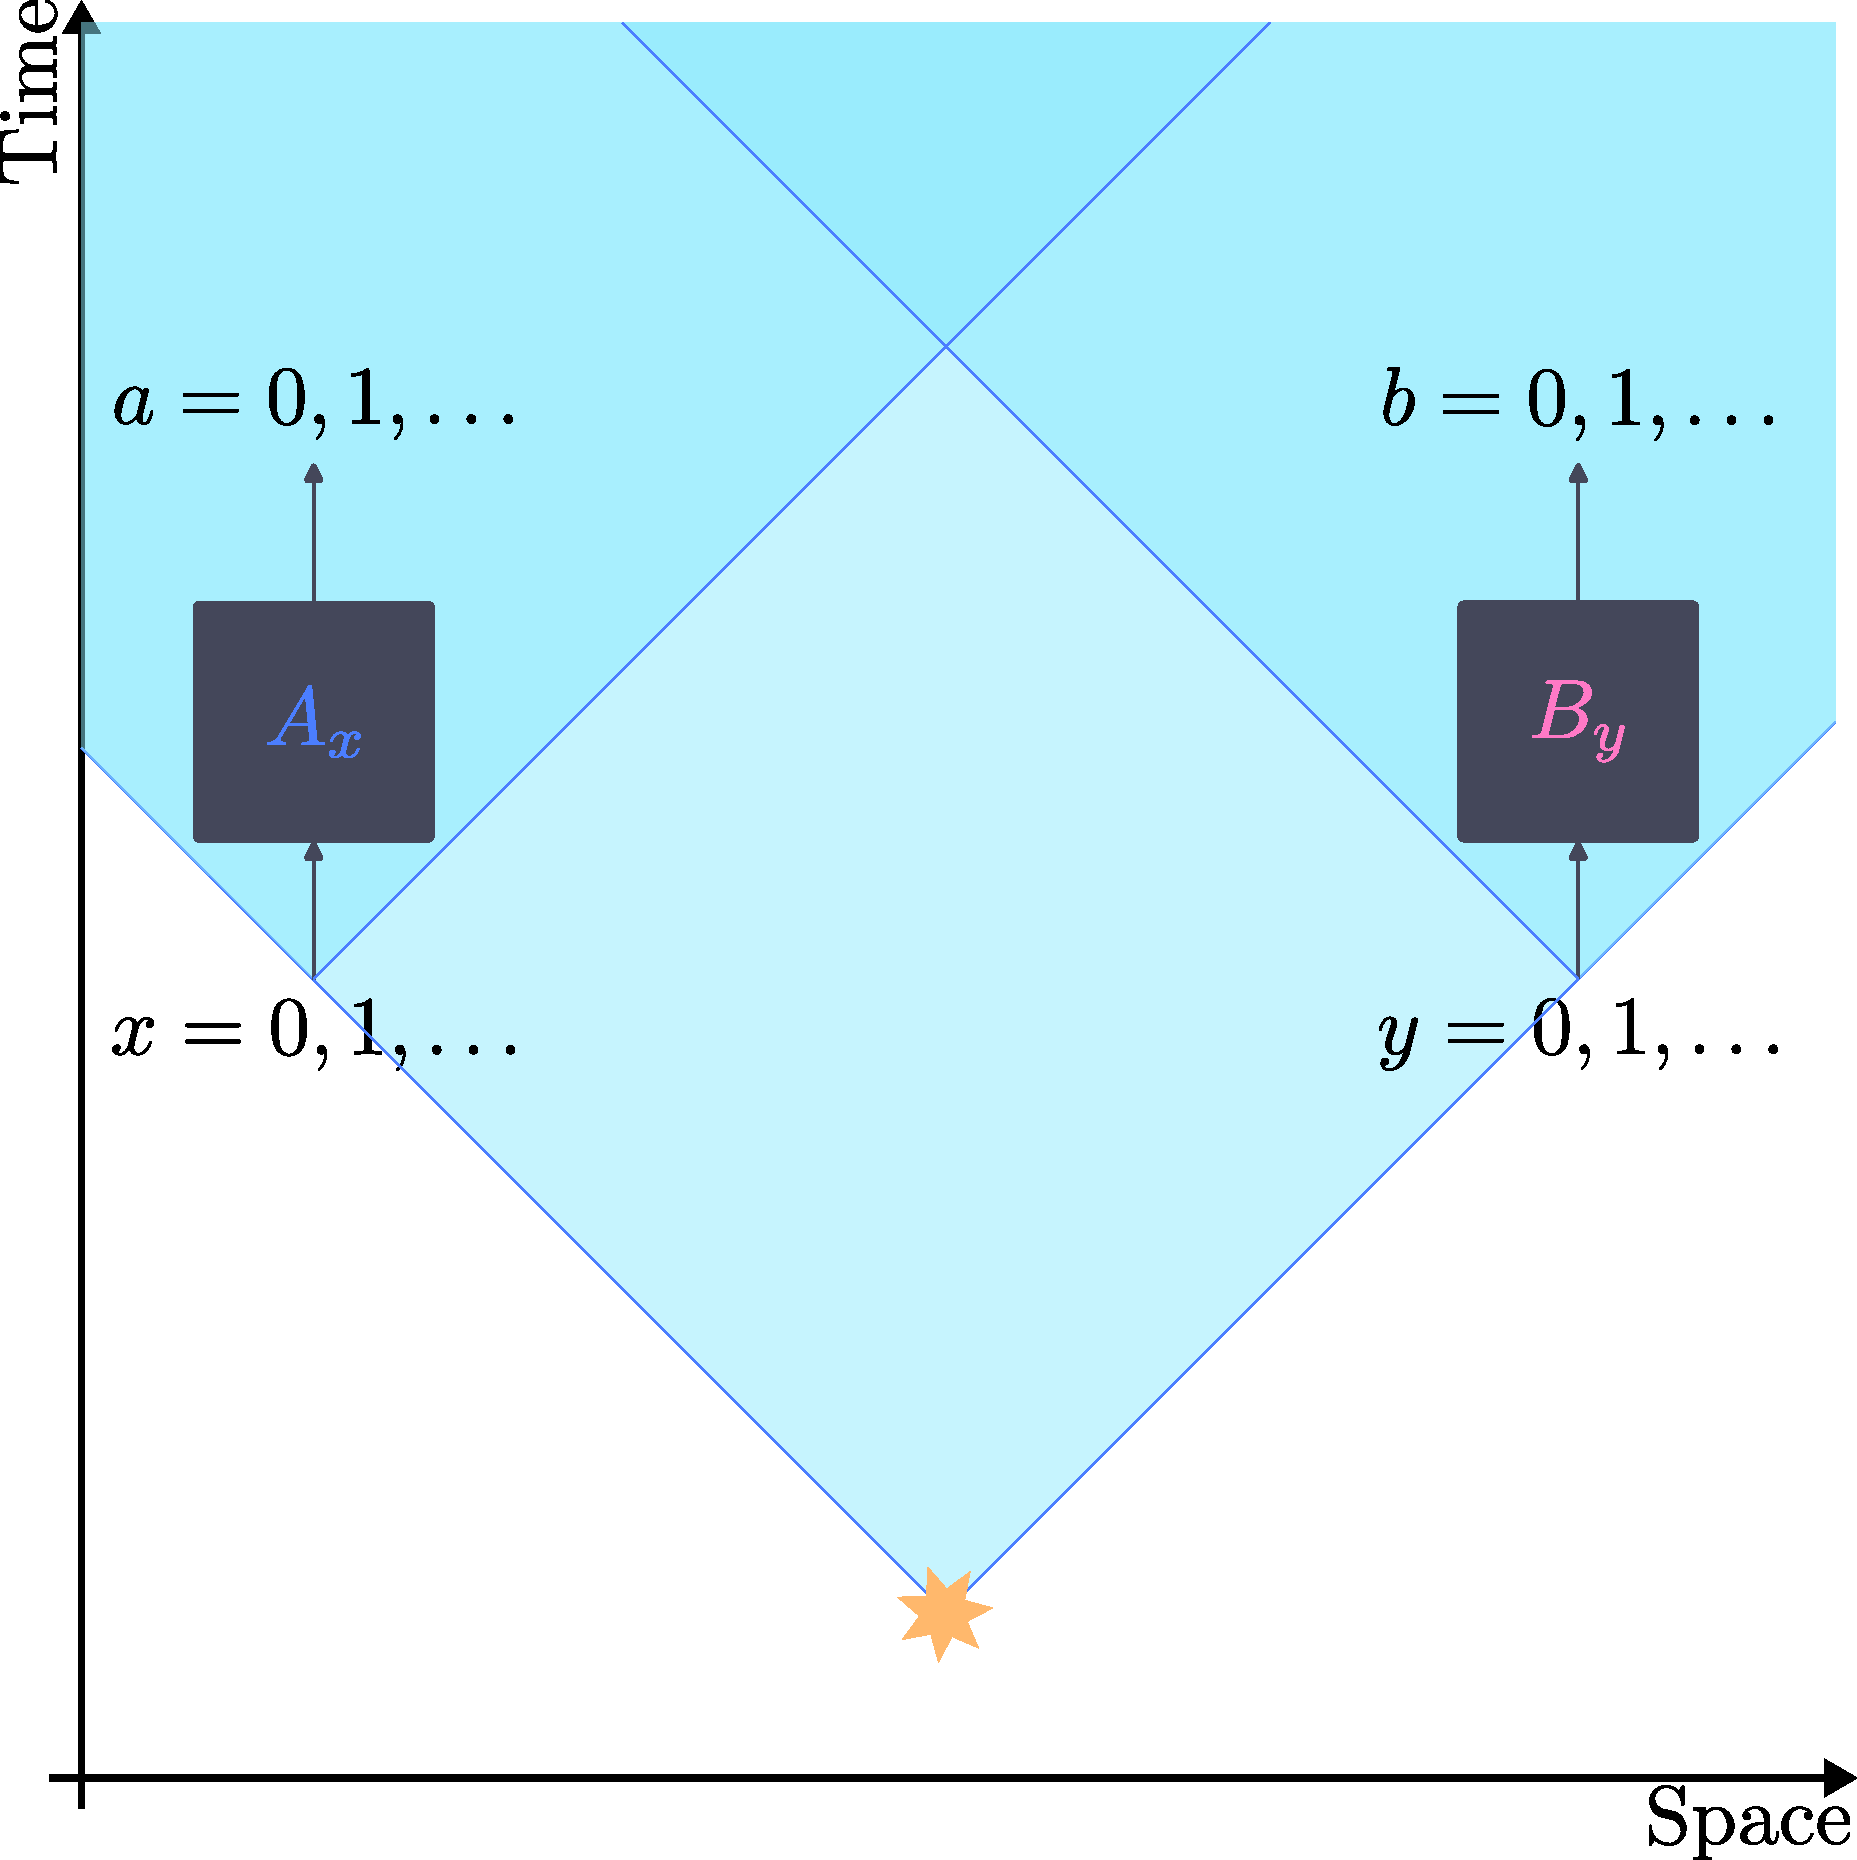
\includegraphics[width=0.95\textwidth]{chapters/overview/img/belltest.pdf}
	\end{center}
	\caption{Bell game. A source (yellow star) emits a particle-pair, one send to Alice (left) and one to Bob (right). Alice chooses an input $x$ and obtains an output $a$. Bob selects an input $y$ and records the output $b$. The blue areas represent light-cones of different events. For a Bell test to be valid, the measurement outcome of a party has to be recorded outside the light-cone triggered by the other party's choice of setting. }
	\label{fig:belltest}
\end{figure}


\section{Non-signalling correlations}

\textit{Non-signalling} correlations are correlations respecting a single assumption: the measurement choice of one party can not influence the outcome of the other party's measurement.
When Alice and Bob are space-like separated, this assumption is trivially enforced by special relativity, i.e. no information can be transmitted faster-than-light.

Formally, non-signalling correlations are correlations for which the local marginals of a party are independent of the other party's measurements choice. 
Mathematically, such correlations satisfy
\begin{equation}
	\begin{split}
		\sum_b p(ab|xy) = \sum_b p(ab|xy') = p(a|x), \quad &\forall\,a,x,y,y' \\
		\sum_a p(ab|xy) = \sum_a p(ab|x'y) = p(b|y), \quad &\forall\,b,x,x',y.
	\end{split}
	\label{eq:non-signalling}
\end{equation}

\pagebreak 

\section{Local and non-local correlations}

\textit{Local correlations} are fully characterised from the local system of Alice and Bob, i.e. they are not influenced by actions outside the light cone.
This type of correlation accounts for some hypothetical shared hidden information between the two parties.
Since Alice and Bob's particles were in contact in the past, outcomes of their measurements can be influenced by some past factors, available locally to both parties' systems but possibly unobservable, i.e. \textit{hidden}.
These past factors are often called \textit{local-hidden variables} and are represented by $\lambda$.
Given that $\lambda$ can be distributed according to $q(\lambda)$ we formally defined local correlations as any correlation that can be decomposed as
\begin{equation}
	p(ab|xy) = \int_\lambda \mathrm{d}\lambda \, q(\lambda) p(a|x,\lambda) p(b|y,\lambda).
	\label{eq:local}
\end{equation}
One assumption we made in writing this decomposition is the \textit{freedom of choice} of both parties' measurements, that is $x$ and $y$ are independent of $\lambda$.

Interestingly, any local correlation can be written as a convex sum of deterministic local strategies, $p_D(ab|xy)=p_D(a|x)p_D(b|y)$, for which the output only depends on the input, following
\begin{equation}
	p(ab|xy) = \sum_{p_D \in \mathcal{L}_\text{Det}} c_{p_D} p_D(ab|xy)
	\label{eq:polytope}
\end{equation}
with $c_{p_D}\geq 0$ and $\sum c_{p_D} = 1$. 
Here $\mathcal{L}_\text{Det}$ is the set of all deterministic local strategies.
From the previous decomposition, it follows that the convex sum of local strategies is also local. 
Geometrically, the set of local correlations is the convex hull of a finite number of deterministic strategies, which is a convex polytope, the \textit{local polytope}.

\medbreak

\textit{Non-local} correlations are defined as any correlation that does not admit a decomposition in the form of \refeq{local}.
Such correlations can thus not be explained by means of local-hidden variables. 
Note that this is the case for some non-signalling correlations as correlations satisfying \refeq{non-signalling} do not necessarily admit a decomposition of the form \refeq{local}.
However, local correlations fulfill the non-signalling assumption. 
See \cite{Brunner14,Scarani2019} for a review on Bell nonlocality.

\section{Quantum correlations}

\textit{Quantum correlations} occur when Alice and Bob's particles are described by a quantum state $\rho_{AB}$.
Generally, this quantum state is a mixed state laying in the Hilbert space $\mathcal{L}(\mathscr{H}^{AB} = \mathscr{H}^{A} \otimes \mathscr{H}^B)$.
For measurement choices $x,y$, quantum correlations are given by the Born rule
\begin{equation}
	p(ab|xy) = \trr{\rho_{AB} M^a_x \otimes M^b_y} \quad \forall\,a,b,x,y
	\label{eq:Born}
\end{equation}
where $M^a_x$ are the \acrfull{povm} elements of the observable $A_x$ associated with outcome $a$, and similarly for Bob with the \acrshort{povm} $M^b_y$ for the observable $B_y$ and the outcome $b$.

\medbreak

Quantum correlations satisfy the non-signalling assumption, but are not necessarily local.
In order to obtain non-local quantum correlations, Alice and Bob must share an entangled state as the correlation produced by a separable state $\rho_{AB}^{\mathrm{sep}} = \sum_i c_i \rho^A_i \otimes \rho^B_i$,
\begin{equation}
	\begin{split}
		p(ab|xy) &= \trr{\rho_{AB}^{\mathrm{sep}} \, M^a_x \otimes M^b_y} \\
				 &= \sum_i c_i\, \trr{(\rho^A_i \otimes \rho^B_i) (M^a_x \otimes M^b_y)} \\
				 &= \sum_i c_i\, \trr{\rho^A_i M^a_x \otimes \rho^B_i M^b_y} \\
				 &= \sum_i c_i\, p_i(a|x)\, p_i(b|y)
	\end{split}
\end{equation}
is of the form \refeq{polytope} and thus local.
Entanglement can therefore be detected solely from the observations of non-local correlations, given that the non-signalling assumption is enforced.

\section{Bell inequalities}

In his 1964 paper, John Bell proposed bounds satisfied by correlations that can be described with local-hidden variables theories~\cite{Bell1964}.
Today, these bounds are known as \textit{Bell inequalities}.
Facets of the local polytopes are examples of such Bell inequalities.
When a Bell inequality is not satisfied by some correlations, we observe a \textit{Bell violation}.
Consequently, violating a Bell inequality proves the presence of non-locality and, therefore, of entanglement.

\medbreak

The most general expression of a Bell inequality $\mathcal{I}$ on some correlation $\mathbf{P}$ is
\begin{equation}
	\mathcal{I}(\mathbf{P}) = \sum_{a,b,x,y}c_{abxy} p(ab|xy) \leq \beta_L
	\label{eq:bell_inequality}
\end{equation}
where $\beta_L$ is the \textit{local bound}, i.e. the maximum Bell score such that $\mathbf{P}$ satisfies \refeq{local}.

\section{CHSH inequality}

\acrfull{chsh}, in a effort to experimentally test Bell's theorem, proposed a more specific version of Bell's game and inequality~\cite{Clauser1969}.
The game, today known as the \textit{\acrshort{chsh} game}, limits Alice and Bob to two dichotomic measurements, $A_0,A_1$ for Alice and $B_0,B_1$ Bob, with outcomes $a,b\in\{\pm 1\}$. 
A well-suited Bell inequality for this game is the \acrshort{chsh} inequality 
\begin{equation}
	S = \left | \mean{A_0 B_0} + \mean{A_0 B_1} + \mean{A_1 B_0} - \mean{A_1 B_1}  \right | \leq 2
	\label{eq:CHSH}
\end{equation}
where $S$ is the \textit{CHSH score}, and $\mean{A_x B_y} = \sum_{a,b} ab\,p(ab|xy)$ expresses a \textit{correlator} -- quantifying how correlated are the outcomes of two measurements.
Note that correlators of a quantum state $\rho_{AB}$ are defined using Born rule, $\mean{A_x,B_y} = \trr{(A_X \otimes B_y)\rho_{AB}}$.
It is convenient to define the \acrshort{chsh} operator, a Bell operator,
\begin{equation}
	\mathcal{B}_{\mathrm{CHSH}} = A_0 \otimes \left( B_0 + B_1 \right) + A_1 \otimes \left( B_0 - B_1 \right)
	\label{eq:CHSH_operator}
\end{equation}
from which the \acrshort{chsh} score can be obtain using $S = \left| \trr{\mathcal{B}_\mathrm{CHSH}\, \rho_{AB} } \right|$.

\medbreak

The inequality \refeq{CHSH} can be used to prove the non-local nature of quantum mechanics. 
Consider the $\ket{\psi^-}$ Bell state, also known as the \textit{singlet} state, shared between Alice and Bob, and the measurements
\begin{equation}
	\begin{split}
		A_0 = \sigma_z, \quad & \quad A_1 = \sigma_x \\
		B_0 = \frac{\sigma_z+\sigma_x}{2}, \quad &\quad B_1 = \frac{\sigma_z - \sigma_x}{2}.
		\label{eq:CHSH_measurement}
	\end{split}
\end{equation}
Computing the \acrshort{chsh} score from these resources yield $S=2\sqrt{2}$ which violates the inequality.
It can also be proven that $2\sqrt{2}$ is the maximum \acrshort{chsh} violation achievable using quantum resources~\cite{Tsirelson1980}.

\chapter{Quantum information}
\label{chapter:quantumInfo}

The emergence of quantum information and the second quantum revolution can be attributed to the discovery of quantum entanglement.
Indeed, if quantum mechanics revolutionized technology by leveraging quantum proprieties to process classical information, mostly thanks to the invention of the transistor, there is now a shift to control individual quantum objects and use them as carrier of information.
Quantum information already have numerous technological applications, from quantum computing to quantum cryptography, quantum simulation or quantum sensing to name a few.
For an introduction on most quantum information concepts see \cite{Nielsen2012}.

\section{Device-independent quantum information processing}

Quantum information processing relies heavily on quantum entanglement.
It is then necessary to certify that a proposed implementation carries out some form of entanglement.
A possible approach is to use quantum state tomography, which allows to reconstruct the density matrix of a quantum state~\cite{MauroDAriano2003}.
Another possibility is to use entanglement witnesses, characterizing the \textit{closeness} of state to a target quantum state using specific operators, see e.g. \cite{Bru2002}.
On the downside, these two methods require precisely calibrated measurement devices, which is a major experimental challenge.

To circumvent this problem, one can use a \textit{device-independent} approach, in which all the quantum devices used, both sources and measurement apparatus, are considered as black-boxes, i.e. no assumption is made on their inner working.
As we saw in the previous chapter, a Bell inequality violation certifies the non-local nature of tested correlations and asserts the presence of entanglement .
Hence, a Bell violation is a device-independent certification of entanglement, as it does not require any assumption on how the tested correlations were obtained, i.e. the inputs $x,y$ and outputs $a,b$ are treated as pure mathematical objects with no specific physical nature.
Notice however, that such certification still requires some assumption on the Bell test itself, as measurement independence and a space-like separation between the parties' measurement events are required.

\medbreak

The device-independent approach advances beyond the simple certification of entanglement and is at the core of complex quantum information technologies.
In this thesis we focus on two device-independent protocols.
First, we study self-testing, the most fundamental device-independent protocol, enabling the device-independent certification of specific states and measurements.
Then, we focus on \acrfull{DIQKD}, one of the most peculiar application of the device-independent framework, allowing two parties to share a secret key whose secrecy is guaranteed without making assumptions on the quantum devices used to produce that key.
Another notable device-independent protocol outside the scope of this thesis is the device-independent generation of random numbers of certified quantum origin~\cite{Acin2016,Liu2018}.
%Some more device-independent protocols are build on top of these protocols, e.g. device-independent verifiable blind quantum computing uses self-tests to verify that a computation has been performed correctly on a remote quantum computer~\cite{Hajdusek2015,McKague2016,Reichardt2013}.


\section{Self-testing}

Introduced by Mayers and Yao, self-testing is the cornerstone of device-independent protocols~\cite{Mayers2004}.
It finds its use when a classical client, with access to multiple black-boxes, would like to certify that these boxes performed specific measurements on a specific shared quantum state producing non-local correlations.
Each boxes has some inputs the client can choose freely, and some outputs they can record, that together form some correlations, similarly to a Bell game.
Self-testing protocols test these correlations against a Bell inequality crafted to certify the presence of a specific state and measurements.
More precisely, the maximum violation of some Bell inequality can only be achieved by a particular family of correlations, that necessary originates form a specific state and measurements.
The first self-testing protocol uses the \acrshort{chsh} inequality to certify the presence of maximally entangled two-qubit states~\cite{Mayers2004}. 
New protocols then extended self-testing, notably to all pure bipartite entangled two-qubit states~\cite{Yang2013,Bamps2015}, and even to any pure bipartite entangled state~\cite{Coladangelo2017}. 
For a in-depth review on self-testing, see \cite{Supic2019}.

\medbreak

This device-independent approach is crucial when the devices used to generate the state and perform the measurement for a quantum information processing task are partially unknown, uncharacterised or untrusted.
Therefore, self-testing was extended to device-independent quantum key distribution~\cite{Mayers2004}, verifiable blind quantum computing~\cite{Reichardt2013,Hajdusek2015,McKague2016}, certify blocks of quantum computers~\cite{Magniez2006,Sekatski2018}, or certify a quantum network link~\cite{Bancal2021}.
However, it is worth noting that for some device-independent protocols, correlations can be directly and more efficiently used, without resorting to self-testing.

\medbreak

Originally, self-testing aims at certifying exactly a given state and measurements thanks to the maximum violation of a Bell inequality, only achievable by specific correlations~\cite{Mayers2004}.
Experimentally, this is challenging as noises and losses introduce errors.
Moreover, finite number of repetition rounds lead to statistical uncertainties on the correlations.
To circumvent these issues, \textit{robust self-testing} has been introduced as a mean to approximate a self-test certificate~\cite{Kaniewski2016}.
Robust self-testing guarantees that if a sufficiently high Bell violation is observed, the state and measurements are \textit{close} to the ones we want to certify.
More precisely, from a high enough violation, one can expect to \textit{extract}, from the actual state, a state close to the target one.
Robust self-testing protocols were developed to decrease the requirement on the Bell violation while maintaining a certain closeness to the state to certify~\cite{Bancal2015,Kaniewski2016,Kaniewski2017,Valcarce2022}.

\section{Device-independent quantum key distribution}

As recent advances in quantum computing threaten the security of our current encryption algorithm~\cite{Shor1994,Gouzien2021,Gouzien2023}, more-than-ever is the need for stronger cryptographic protocols. 

One approach is \textit{post-quantum cryptography} (PQC), new classical cryptography protocols that are resistant to known quantum attacks.
PQC is convenient as it does not require new infrastructure, i.e. classical computers and communication links are sufficient. 
However, a major drawback is a poor long-term security; information encrypted using PQC can be stored for years until new quantum attacks that can break the encryption scheme are developed. 
Furthermore, mathematical flaws in these protocols can be discovered, ruling out their security.
This recently happened to a protocol short-listed by the NIST as a candidate for PQC~\cite{Castryck2022}.
For an overview on the current state of PQC see e.g. the recent report by the European Union Agency for Cybersecurity~\cite{EUAC2021}.

Another approach is \acrfull{QKD}, allowing two parties connected by a quantum channel to share a secret key~\cite{Bennett84,Ekert1991,Gisin2002,Scarani2009}.
An important aspect of \acrshort{QKD} is that it does not rely on computational assumptions.
Instead, it leverages the fundamental laws of physics to guarantee, in principle, an unconditional security~\cite{Shor2000,Mayers2001}.
Moreover, the no-cloning theorem forbids a malicious actor to create an independent and identical copy of the information send during a \acrshort{QKD} protocol.
This gives \acrshort{QKD} an infinite long-term security.
It is worth noting that quantum key distribution and PQC are not in competitions with each other as replacements for classical cryptography, rather, they are complementary~\footnote{QKD protocols require an authenticated channel of communication. PQC is a natural candidate to perform this authentication.}.

\medbreak 

First \acrshort{QKD} protocols were \textit{prepare-and-measure} protocols~\cite{Bennett84,Grosshans2002,Grosshans2003}.
In these protocols Alice would send information encoded in a quantum state to Bob.
Thanks to the no-cloning theorem and to the uncertainty principle, attacks performed by an eavesdropper to gain information on the encoded message would unavoidably lead to detectable disturbances.
Alice and Bob could thus detect the eavesdropper and abort the protocol.

Another approach to \acrshort{QKD} is entanglement-based protocols~\cite{Ekert1991}.
In this case, Alice and Bob generate a key from the outcomes of  measurements they perform on a shared entangled signal they receive.
Intuitively, when using a bipartite maximally entangled state, the outcomes of Alice and Bob are fully correlated and completely random.
Therefore, as the generated outcomes are identical and unpredictable on both side, they can be used to define a key.

\medbreak

The security of QKD protocols relies on the following assumptions
\begin{itemize}
	\item 1. The devices used to generate the key and to attack the protocol behave according to quantum theory,
	\item 2. There is no information leakage out of Alice and Bob systems, e.g. Alice and Bob are each in a hermetic laboratory,
	\item 3. Alice and Bob have access to random numbers,
	\item 4. The classical devices used to process classical information are trusted 
	\item 5. The quantum devices used to prepare the state and perform measurements are perfectly calibrated and behave predictably.
\end{itemize}

\medbreak

The level of trust in cryptography is inherently limited by the trust we place on the assumptions our cryptographic protocols rely on. 
To address this limitation, it is highly desirable to remove the assumption that quantum devices are trustworthy.
Indeed, the devices or the apparatus composing these devices may be compromised by third-party producers.
A famous example of such interference on classical system is the cryptographic devices sold by Crypto AG which were bugged by the Central Intelligence Agency~\cite{Miller2020}.
However, even considering an honest manufacturer, the quantum devices implementing QKD are hard to build and will always contain noises and losses~\cite{Diamanti2016,Xu2020}.
Subsequently, QKD implementations inevitably mismatch with the theoretical models on which the security proofs are based. 
Moreover imperfections, especially the ones occurring in single-photon detectors, have been successfully exploited to attack QKD protocols~\cite{Fung2007,Lydersen2010,Gerhardt2011,Weier2011}. 
For a review on quantum hacking, with attack examples, refer to \cite{Lo2014}.

\medbreak

To overcome all of these implementation-related challenges, \acrfull{DIQKD} has been developed~\cite{Acin2007,Vazirani2014,ArnonFriedman2018}.
\acrshort{DIQKD} is a family of more secure quantum key distribution protocols in which the assumption on the inner working of the quantum devices is dropped.
Instead, DIQKD security proofs rely solely on the classical outcomes of measurements on a shared system, both of which are considered as \textit{black-boxes}.
Crucially, DIQKD protocols will simply abort in the presence of exploitable imperfections, which are always appearing in the collected outcomes.

\medbreak

From a maximal violation of the CHSH inequality the singlet state and specific measurements can be self-tested, and therefore, guaranteeing that two parties can have correlated outcomes, unknown to a third party.
Intuitively, DIQKD can be built on top of self-tests; the CHSH score asses the presence of the required resources from which a security proof on the distributed key is derived.
However, this self-tests-based approach leads to performance far from practical applications~\cite{Fu2018,Kundu2022}.
Hence, for better efficiency, the security proof of most protocols is directly based on the CHSH score, or, for even better performance, directly on the observed correlations~\cite{Pironio2009,Ho2020,Sekatski2021,Woodhead2021,Brown2021}.
